% This file was created by matlab2tikz.
%
\definecolor{mycolor1}{rgb}{0.89412,0.10196,0.10980}%
\definecolor{mycolor2}{rgb}{0.21569,0.49412,0.72157}%
%
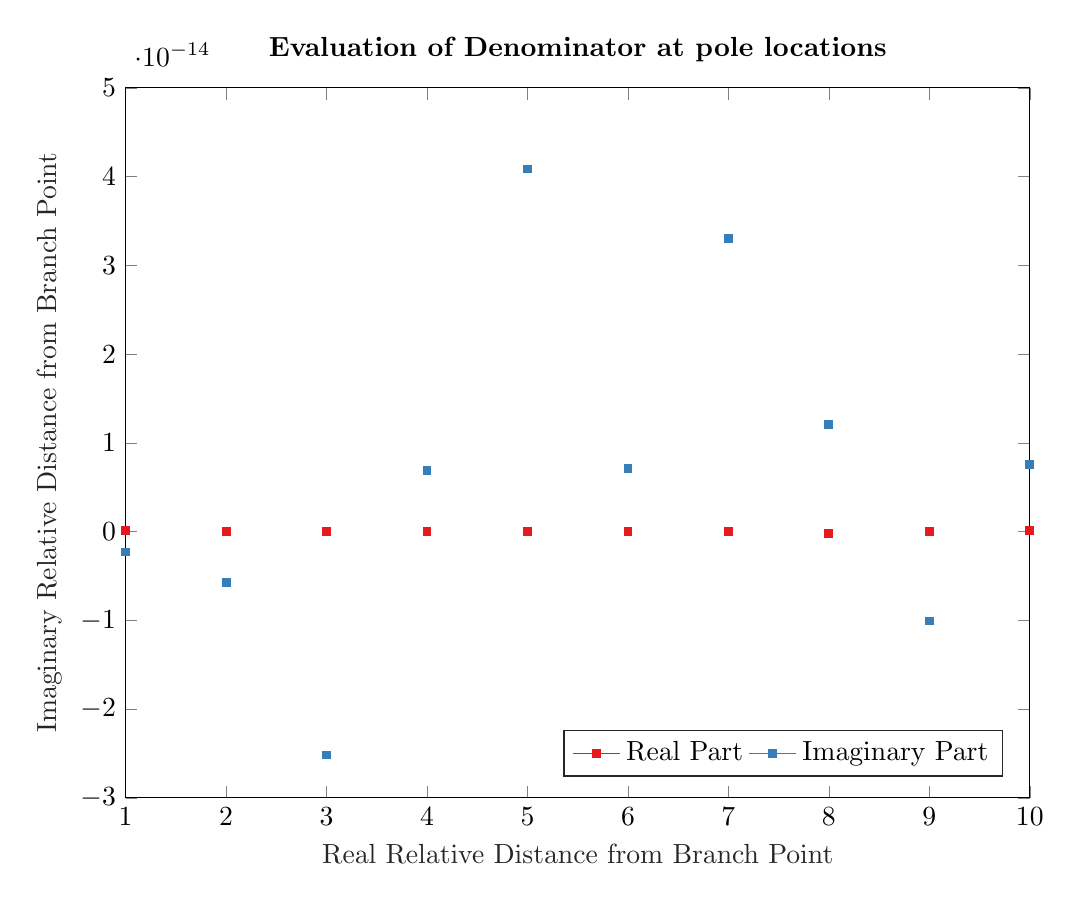
\begin{tikzpicture}

\begin{axis}[%
width=4.521in,
height=3.55in,
at={(0.758in,0.497in)},
scale only axis,
xmin=1,
xmax=10,
xlabel style={font=\color{white!15!black}},
xlabel={$\textrm{Real Relative Distance from Branch Point}$},
ymin=-3e-14,
ymax=5e-14,
ylabel style={font=\color{white!15!black}},
ylabel={$\textrm{Imaginary Relative Distance from Branch Point}$},
axis background/.style={fill=white},
title style={font=\bfseries},
title={Evaluation of Denominator at pole locations},
legend style={at={(0.97,0.03)}, anchor=south east, legend columns=2, legend cell align=left, align=left, draw=white!15!black}
]
\addplot [color=mycolor1, draw=none, mark size=1.4pt, mark=square*, mark options={solid, fill=mycolor1, mycolor1}]
  table[row sep=crcr]{%
1	1.11022302462516e-16\\
2	0\\
3	0\\
4	0\\
5	0\\
6	0\\
7	0\\
8	-2.22044604925031e-16\\
9	0\\
10	1.11022302462516e-16\\
};
\addlegendentry{Real Part}

\addplot [color=mycolor2, draw=none, mark size=1.4pt, mark=square*, mark options={solid, fill=mycolor2, mycolor2}]
  table[row sep=crcr]{%
1	-2.28940130742039e-15\\
2	-5.74171786504873e-15\\
3	-2.51691029129475e-14\\
4	6.87123968834413e-15\\
5	4.08596767531577e-14\\
6	7.14706072102445e-15\\
7	3.30430127704062e-14\\
8	1.21014309684142e-14\\
9	-1.00752739484733e-14\\
10	7.59114993087451e-15\\
};
\addlegendentry{Imaginary Part}

\end{axis}
\end{tikzpicture}%